\chapter{Lie theory and Jacobi diagrams}
\label{ch:lie-theory-and-jacobi-diagrams}

The fundamental theorem of Vassiliev invariants states that the bialgebra of Vassiliev invariants can be broken up into nice combinatiorial weight systems. So to understand \(\mathcal{V}\) it suffices to understand \(\mathcal{W}\), or equivalently its dual \(\mathcal{A}\). There is a hint that the structure of \(\mathcal{A}\) may relate to Lie algebras.

\section{Jacobi diagrams}

This side of the story reframes the bialgebra \(\mathcal{A}\) as an isomorphic bialgebra known as the algebra of Jacobi diagrams to illuminate the Lie theory connections.

\begin{definition}
	A \textbf{unitrivalent diagram} is a unitrivalent graph (with loops and multiple edges allowed) with the following additional data:
	\begin{itemize}
		\item each trivalent vertex has a fixed cyclic order of incident edge-connections,
		\item the set of univalent vertices has a fixed cyclic order.
	\end{itemize}
	The vector space of unitrivalent diagrams is denoted \(\mathcal{T}\).
\end{definition}

When drawing unitrivalent diagrams, there are two notation conventions. Firstly, the fixed cyclic order of the univalent edges is specified by drawing them connected to a circle (the cyclic order is induced by traversing the circle anticlockwise).  Secondly, all the trivalent vertices are taken with the anticlockwise cyclic ordering unless an arrow around that vertex indicates otherwise.

In particular, from the first point, all chord diagrams are unitrivalent diagrams with only univalent vertices (the chord ends). Further examples of unitrivalent diagrams would be
\[
	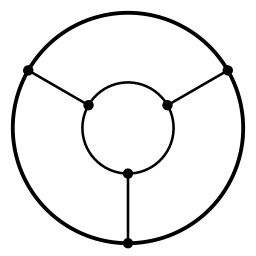
\includegraphics[width=0.13\textwidth, valign=c]{graphics/unitrivalent_diagram_example_1.pdf} \ ,
	\quad
	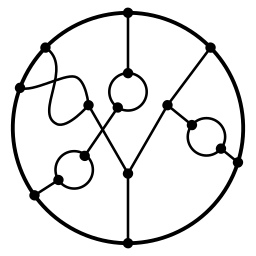
\includegraphics[width=0.13\textwidth, valign=c]{graphics/unitrivalent_diagram_example_2.pdf}
	\in \mathcal{T}.
\]

\begin{definition}
	The \textbf{STU relation} is the relation
		\begin{equation}
			\label{eq:STU}
			\tag{\stu}
			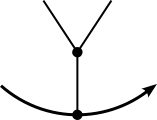
\includegraphics[width=0.10\textwidth, valign=c]{graphics/stu_relation_s.pdf}
			\quad
			=
			\quad
			\includegraphics[width=0.10\textwidth, valign=c]{graphics/stu_relation_t.pdf}
			\quad
			-
			\quad
			\includegraphics[width=0.10\textwidth, valign=c]{graphics/stu_relation_u.pdf}.
		\end{equation}
\end{definition}

As usual, this is not an individual relation but a class of relations, true in any diagrams that are identical except for the parts shown.

Note that the for the chord diagrams inside the algebra of Jacobi diagrams, the \ref{eq:STU} relations imply the \ref{eq:4T} relations, as
	\[
		\adjustbox{valign=c}{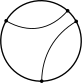
\includegraphics[width=0.115\textwidth]{graphics/four_term_from_stu_north.pdf}}
		\ - \
		\adjustbox{valign=c}{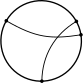
\includegraphics[width=0.115\textwidth]{graphics/four_term_from_stu_south.pdf}}
		\ = \
		\adjustbox{valign=c}{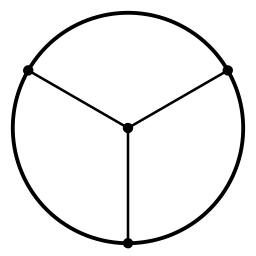
\includegraphics[width=0.12\textwidth]{four_term_jacobi_diagram.pdf}}
		\ = \
		\adjustbox{valign=c}{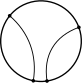
\includegraphics[width=0.115\textwidth]{graphics/four_term_from_stu_west.pdf}}
		\ - \
		\adjustbox{valign=c}{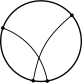
\includegraphics[width=0.115\textwidth]{graphics/four_term_from_stu_east.pdf}}\ .
	\]

\begin{definition}
	The algebra \(\mathcal{J}\) of Jacobi diagrams is the vector space \(\mathcal{T} / \ref{eq:STU}\), with the product \(\connect\) defined the same way as it was for chord diagrams.
\end{definition}

This is well-defined: the proof of Proposition \ref{prop:connected-sum-well-defined} showed that the product \(\connect\) being well-defined on \(\mathcal{A}\) was a consequence of the \ref{eq:4T} relations, which are implied by the \ref{eq:STU} relations. From the \ref{eq:STU} relations, we may deduce the following other relations which hold in \(\mathcal{J}\).

\begin{proposition}
	The following relations are consequences of the \textup{\ref{eq:STU}} relation in \(\mathcal{J}\):
	\begin{enumerate}
		\item The \textbf{AS relation} (antisymmetry relation),
			\begin{equation}
				\label{eq:AS}
				\tag{\as}
				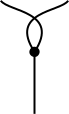
\includegraphics[width=0.05\textwidth, valign=c]{graphics/as_relation_a.pdf}
				\quad
				=
				\quad
				-
				\includegraphics[width=0.05\textwidth, valign=c]{graphics/as_relation_s.pdf}.
			\end{equation}
		\item The \textbf{IHX relation},
			\begin{equation}
				\label{eq:IHX}
				\tag{\ihx}
				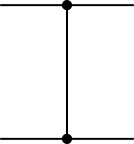
\includegraphics[width=0.10\textwidth, valign=c]{graphics/ihx_relation_i.pdf}
				\quad
				=
				\quad
				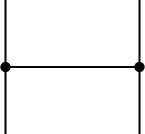
\includegraphics[width=0.10\textwidth, valign=c]{graphics/ihx_relation_h.pdf}
				\quad
				-
				\quad
				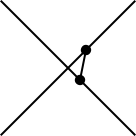
\includegraphics[width=0.10\textwidth, valign=c]{graphics/ihx_relation_x.pdf}.
			\end{equation}
	\end{enumerate}
\end{proposition}

\begin{proof}
	\begin{enumerate}
		\item
			Take two diagrams which differ only by \ref{eq:AS} at one (trivalent) vertex. If the vertex at which the \ref{eq:AS} relation resides is adjacent to a univalent vertex (i.e. touches the outer circle), then this is immediate from applying \ref{eq:STU} to both diagrams at that vertex.
			\[
				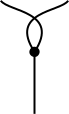
\includegraphics[width=0.05\textwidth, valign=c]{graphics/as_relation_a.pdf}
				\quad
				=
				\quad
				\includegraphics[width=0.10\textwidth, valign=c]{graphics/stu_relation_u.pdf}
				\quad
				-
				\quad
				\includegraphics[width=0.10\textwidth, valign=c]{graphics/stu_relation_t.pdf}
				\quad
				=
				\quad
				-
				\includegraphics[width=0.05\textwidth, valign=c]{graphics/as_relation_s.pdf}.
			\]

			If the vertex is not immediately adjacent to a univalent vertex, then it has some \(d\) vertices `in the way'. By applying \ref{eq:STU} to those vertices yields a sum of \(2^{d}\) diagrams, all identical except for differing by \ref{eq:AS}, now on a vertex adjacent to a univalent vertex.

		\item
			A similar argument applies. If one of the two vertices of the \ref{eq:IHX} is adjacent to the circle, then the result is a direct consequence of an \ref{eq:STU} on each of the vertices, then some applications of \ref{eq:AS}. Otherwise, some \ref{eq:STU}s are required first.
			% TODO: (time permitting) figures.
\end{enumerate}
\end{proof}

\begin{proposition}[Generalised \ref{eq:IHX}]
	\label{lem:generalised-ihx}
	The following holds in \(\mathcal{J}\) for any subgraph consisting of trivalent vertices that can be inserted into the grey box.
	\[
		\sum_{i = 0}^{m}\
		\def\svgscale{0.3}
		\raisebox{-34pt}{\input{graphics/generalised_ihx_left.pdf_tex}}
		\quad
		=
		\quad
		\sum_{i = 0}^{n}\
		\def\svgscale{0.3}
		\raisebox{-34pt}{\input{graphics/generalised_ihx_right.pdf_tex}}
	\]
\end{proposition}

The result is standard, see Chapter 5.2 of \cite{introduction-to-vassiliev-invariants} for a proof. A corollory is the following result, which will be important later.

\begin{proposition}
	\label{prop:linear-jacobi-diagrams-cyclically-invariant}
	If the univalent vertices of a Jacobi diagram are ordered linearly rather than cyclically, all linear orders that respect a given cyclic order are equivalent.
\end{proposition}

\begin{proof}
	Let us draw the linearly ordered Jacobi diagrams on a line rather than a circle and let the univalent edge ordering be given by the order on the line. It suffices to prove that we can move the univalent vertex in the first place to the last place via the relations in \(\mathcal{A}\). Let us call this first univalent vertex of the original diagram the marked vertex, as its position will later change when relations are applied.

	By \ref{eq:STU}, the original diagram is equal to the diagram with the marked vertex moved into the second place, plus a diagram in which the marked vertex is now a trivalent vertex and attached above what was the second (but is now the first) univalent vertex.
	\[
		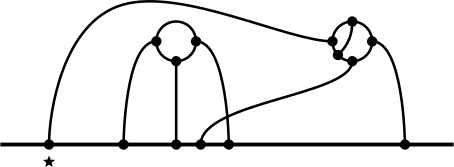
\includegraphics[width=0.25\textwidth, valign=c]{graphics/long_jacobi_diagram_example.pdf}
		\quad
		=
		\quad
		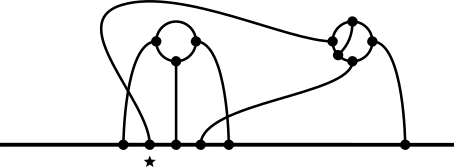
\includegraphics[width=0.25\textwidth, valign=c]{graphics/long_jacobi_diagram_example_t.pdf}
		\quad
		+
		\quad
		\includegraphics[width=0.25\textwidth, valign=c]{graphics/long_jacobi_diagram_example_u.pdf}
	\]
	Repeatedly applying \ref{eq:STU} to move the the marked vertex until reaches the last place, we get
	\[
		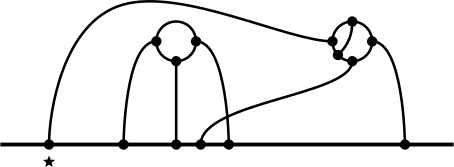
\includegraphics[width=0.25\textwidth, valign=c]{graphics/long_jacobi_diagram_example.pdf}
		\quad
		=
		\quad
		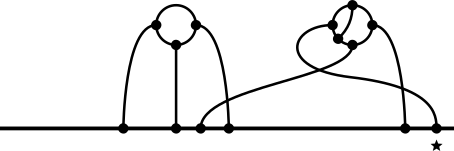
\includegraphics[width=0.25\textwidth, valign=c]{graphics/long_jacobi_diagram_example_final.pdf}
		\quad
		+
		\quad
		\Theta
	\]
	where \(\Theta\) is a sum of terms with the marked vertex now a trivalent vertex attached above each of the other univalent vertices. It suffices to show that \(\Theta\) vanishes.

	We can split \(\Theta\) up based on which connected component the marked vertex now connects to. For connected components other than the connected component of the marked vertex, apply a vertical version of the the generalised \ref{eq:IHX}, where the the whole connected component is inside the grey box except for where the univalent vertices connect to the bottom line. This is the case of the generalised \ref{eq:IHX} where \(n = 0\) and no vertices leave. Hence, the sum vanishes for that connected component.

	This leaves only the terms where the marked vertex connects back to its own connected component. By a generalised \ref{eq:IHX} of the form
	\[
		\sum \includegraphics[width=0.25\textwidth, valign=c]{graphics/long_jacobi_diagram_example_same_cc.pdf}\; ,
		\quad
		\text{this is equal to the diagram}
		\quad
		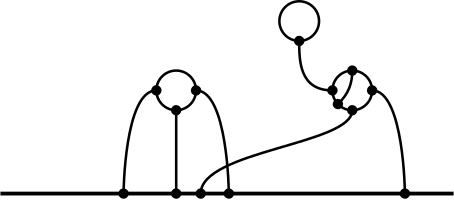
\includegraphics[width=0.25\textwidth, valign=c]{graphics/long_jacobi_diagram_example_lollipop.pdf}.
	\]
	But any diagram with a ``balloon'' vanishes, as applying the \ref{eq:AS} relation to the vertex on the balloon, it is equal to its negative.

	Hence \(\Theta = 0\), completing the proof.
\end{proof}

We have already spoiled the surprise that in the end, \(\mathcal{A}\) and \(\mathcal{J}\) will be isomorphic as bialgebras. In fact, as algebras, this is clearly true so far, as \(\mathcal{J}\) is just a change of basis from \(\mathcal{A}\). Since \(\mathcal{A}\) spans \(\mathcal{J}\), we can attempt to lift the coproduct from \(\mathcal{A}\) directly onto \(\mathcal{J}\).

\begin{proposition}
	The coproduct \(\Delta\) on \(J \in \mathcal{J}\) defined by taking a Jacobi diagram, representing it as a chord diagram via \textup{\ref{eq:STU}}, taking the coproduct in \(\mathcal{A}\), then interpreting the result as a Jacobi diagram via the inclusion of \(\mathcal{A}\) into \(\mathcal{J}\), is also given by the following formula.

	\[\Delta(J) = \sum_{C \subset S} J_{C} \otimes J_{\overline{C}},\]
	where \(S\) is the set of connected components of \(J\), and \(\overline{C} = S \smallsetminus C\).
\end{proposition}

\begin{proof}
	Note that this has the same symbolic form as the coproduct in \(\mathcal{A}\) given in Definition~\ref{def:coproduct-in-chord-diagrams}, but with chords replaced by connected components of Jacobi diagrams. However, when working in \(\mathcal{A} \subset \mathcal{J}\), there are only univalent vertices, so the connected components are exactly the chords. Since \(\mathcal{A}\) forms a basis for \(\mathcal{J}\), and the formula is linear, it extends to all of \(\mathcal{J}\).
\end{proof}

\begin{corollary}
	The primitive elements \(\mathcal{P}(\mathcal{A})\) are the connected Jacobi diagrams.
\end{corollary}

\begin{corollary}
	The bialgebras \(\mathcal{A}\) and \(\mathcal{J}\) are isomorphic.
\end{corollary}

\begin{warning}
	Justified by this isomorphism, we henceforth write \(\mathcal{A}\), for both chord diagrams and Jacobi diagrams.
\end{warning}

\section{Lie algebra weight systems}
Similar diagrammatic relations to \ref{eq:STU}, \ref{eq:AS} and \ref{eq:IHX} satisfied in \(\mathcal{A}\) are appear also in the context of a graphical notation for multilinear maps, a fact which we may exploit to probe \(\mathcal{A}\). Before seeing how, let us review this graphical notation following \cite{wheeling-a-diagrammatic-analogue-of-the-duflo-isomorphism, on-the-rozansky-witten-weight-systems}. This diagrammatic calculus is well-known but it goes by many names: string diagram calculus, Penrose calculus, tensor calculus, diagrammatic calculus for tensors, etc. We call them string diagrams.

A tensor is a multilinear map \(X_{1} \otimes X_{2} \otimes \cdots \otimes X_{n} \to Y_{1} \otimes Y_{2} \otimes \cdots \otimes Y_{m}\), or equivalently (via the canonical isomorphism) an element of the vector space \(X_{1}^{\ast} \otimes X_{2}^{\ast} \otimes \cdots X_{n}^{\ast} \otimes Y_{1} \otimes Y_{2} \otimes \cdots \otimes Y_{m}\). Such a tensor can be represented as a vertex with \(m + n\) unbound directed edges: \(m\) incoming edges decorated by the corresponding vector spaces (in the example above, \(X_{1}, \cdots\)), and \(n\) outgoing edges decordated by \(Y_{1}, \cdots\). For example, the bracket in a Lie algebra \(\mathfrak{g}\) is an element \([\cdot,\cdot] \in \mathfrak{g}^{\ast} \otimes \mathfrak{g}^{\ast} \otimes \mathfrak{g}\), expressed as
\[\def\svgscale{0.3} \input{graphics/bracket_string_diagram.pdf_tex}.\]
It will be obvious from each string diagram what tensor it represents so we can drop the edge labels.

Such a notation is useful because composition of tensors can be expressed graphically by connecting outgoing and incoming legs with the same decoration. Relations can therefore be expressed graphically, for example, the antisymmetry of the bracket \([y, x] = -[x, y]\) becomes
\[
	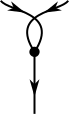
\includegraphics[width=0.05\textwidth, valign=c]{graphics/bracket_antisymmetry_swap.pdf}
	\quad
	=
	\quad
	-
	\includegraphics[width=0.05\textwidth, valign=c]{graphics/bracket_antisymmetry_id.pdf}.
\]
the Jacobi relation \([[x, y], z] + [[y, z], x] + [[z, x], y] = 0\) becomes
\[
	\includegraphics[width=0.10\textwidth, valign=c]{graphics/jacobi_symmetric_xyz.pdf}
	\quad
	+
	\quad
	\includegraphics[width=0.10\textwidth, valign=c]{graphics/jacobi_symmetric_yzx.pdf}
	\quad
	+
	\quad
	\includegraphics[width=0.10\textwidth, valign=c]{graphics/jacobi_symmetric_zxy.pdf}
	\quad
	=
	\quad
	0
\]

Looking at the relations these relations in the tensor algebra \(\mathcal{T}(\mathfrak{g})\), the first solid evidence of Lie-theoretic structure in this story emerges. The antisymmetry of the bracket, drawn as a string diagram looks like a directed version of \ref{eq:AS}. Similarly the string diagram Jacobi relation can be arranged into a directed version of \ref{eq:IHX}.

% TODO: Decide whether we can be bothered to talk about representations also as vertices. We can also just weight systems into U(g) then take traces wrt a rep after.

Furthermore, suppose \(\mathfrak{g}\) is a metric Lie algebra. Then it has an invariant, nondegenerate, bilinear form \(\langle \cdot, \cdot \rangle \in \mathfrak{g}^{\ast} \otimes \mathfrak{g}^{\ast}\). Being nondegenerate, it can be inverted to an element \(c \in \mathfrak{g} \otimes \mathfrak{g}\). This element is known as the casimir. These tensors can be diagrammatically represented as additional bivalent vertices.
\[
	\includegraphics[width=0.06\textwidth, valign=c]{graphics/string_diagram_metric.pdf}
	\qquad \text{and} \qquad
	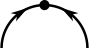
\includegraphics[width=0.06\textwidth, valign=c]{graphics/string_diagram_casimir.pdf}\ .
\]
The bilinear form induces an isomorphism of \(\mathfrak{g}\) and \(\mathfrak{g}^{\ast}\). Diagramatically, this can be used to change the arrow direction on any edge, allowing us to drop the edge arrows from the notation.

Moreover, the invariance of the metric can be written as \(\langle [x, y], z \rangle = \langle [y, z], x \rangle\) which graphically can be represented as cyclic invariance of the contraction of the bracket and the metric
\[
	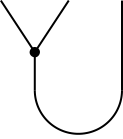
\includegraphics[width=0.08\textwidth, valign=c]{graphics/bracket_metric_cyclic_invariance_bracketxy.pdf}
	\quad
	=
	\quad
	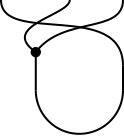
\includegraphics[width=0.08\textwidth, valign=c]{graphics/bracket_metric_cyclic_invariance_permute.pdf}
	\quad
	=
	\quad
	\includegraphics[width=0.08\textwidth, valign=c]{graphics/bracket_metric_cyclic_invariance_bracketyz.pdf}.
\]
A similar argument works for the casimir.

A representation of \(\mathfrak{g}\) on a finite-dimensional vector space \(V\) can be written as a tensor \(\rho \in \mathfrak{g}^{\ast} \otimes V^{\ast} \otimes V\). This takes a new kind of input an output, namely a \(v \in V\) which we denote by a thick line at a shallow angle
\[
	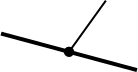
\includegraphics[width=0.11\textwidth, valign=c]{graphics/representation_vertex.pdf}.
\]
That this action be a Lie action,
\[\rho([x, y]) = \rho(x)\rho(y) - \rho(y)\rho(x)\]
is graphically
\[
	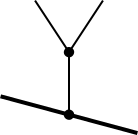
\includegraphics[width=0.1\textwidth, valign=c]{graphics/string_diagram_lie_action_s.pdf}
	\quad
	=
	\quad
	\includegraphics[width=0.1\textwidth, valign=c]{graphics/string_diagram_lie_action_t.pdf}
	\quad
	-
	\quad
	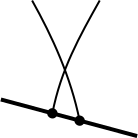
\includegraphics[width=0.1\textwidth, valign=c]{graphics/string_diagram_lie_action_u.pdf}.
\]

%TODO (Zsuzsi) I was missing this sentence below where you first introduced the graphical notation for a representation
Again, arrows are unnecessary on the thick edges corresponding to inputs and outputs of \(V\), as cup and cap vertices similar to the metric and casimir for \(\mathfrak{g}\) are given by the maps
\[f \otimes v \longmapsto f(v) \quad \text{and} \quad 1 \longmapsto \sum_{i} e_{i} \otimes e_{i}^{\ast}.\]

The famous construction of Bar-Natan \cite{on-the-vassiliev-knot-invariants} uses this diagrammatic calculus to take metric Lie algebras and produce weight systems.

\begin{construction}
	\label{cons:lie-algebra-weight-system}
	The construction takes a metric Lie algebra \(\mathfrak{g}\), and produces a map \(W_{\mathfrak{g}}: \mathcal{A} \to \mathcal{U}(\mathfrak{g})\) which is a \(\mathcal{U}(\mathfrak{g})\)-valued weight system. Given further a representation \(\rho\) of \(\mathfrak{g}\) it produces a map \(W_{\mathfrak{g}}: \mathcal{A} \to k\) which is a \(k\)-valued weight system. That is, given \(\mathfrak{g}\) a metric Lie algebra, \(J \in \mathcal{A}\) it produces an element of \(\mathcal{U}(\mathfrak{g})\), and if also given a representation \(\rho\) it produces a scalar. We write \(v\) and \(u\) for the number of trivalent and univalent vertices of \(J\).

	To each trivalent vertex of \(J\), associate a copy of the tensor \([\cdot, \cdot] \in \mathfrak{g}^{\ast} \otimes \mathfrak{g}^{\ast} \otimes \mathfrak{g}\) (see Warning \ref{warn:cyclic-order-of-bracket}). For each edge between trivalent vertices, contract the corresponding tensors along the components corresponding to those half-edges. Where the signature of the components doesn't allow for contraction (both components are covariant, i.e. inputs or both are contravariant, i.e. outputs), contract one of them first with either the metric or the casimir (whichever is allowed by its variance). The resulting tensor has \(u\) components (they may be co- or contra-variant). 

	Contract this tensor with a copy of the casimir along all remaining covariant components. We define the result to be the tensor \(T_{\mathfrak{g}}(J) \in \mathfrak{g}^{\otimes u}\). The linear order of its components must be a linear order that agrees with the cyclic order of the corresponding univalent vertices in \(J\). Define \(W_{\mathfrak{g}}(J)\) to be the projection of this tensor into \(\mathcal{U}(\mathfrak{g})\),
	\[W_{\mathfrak{g}}(J) = [T_{\mathfrak{g}}(J)] \in \mathcal{U}(\mathfrak{g}).\]

	A representation \(\rho: \mathfrak{g} \to \operatorname{Hom}(V)\) of a Lie algebra extends uniquely to a representation of its universal enveloping algebra \(\rho: \mathcal{U}(\mathfrak{g}) \to \operatorname{Hom}(V)\). Define \(W_{\mathfrak{g}, \rho}\) as the trace of \(W_{\mathfrak{g}}(J)\) with respect to this representation,
	\[W_{\mathfrak{g}, \rho}(J) = \operatorname{tr}(\rho(W_{\mathfrak{g}}(J))) \in \mathbb{Q}.\]
\end{construction}

\begin{warning}
	\label{warn:cyclic-order-of-bracket}
	In Construction \ref{cons:lie-algebra-weight-system} when constructing \(T_{\mathfrak{g}}(m)\), the tensor factors in the tensor corresponding to the bracket need to have the unusual cyclic order \((y^{\ast}, x^{\ast}, [x, y]_{\mathfrak{g}})\). This is because its projection into \(\mathcal{U}(\mathfrak{g})\) should obey \ref{eq:STU}, and this is the cyclic order of the trivalent vertex in \ref{eq:STU} (this will become evident in the proof that this construction works).
\end{warning}

\begin{example}
	\label{ex:simple-sl2-computation}
	Take the metric Lie algebra \((\mathfrak{sl}_{2}, \langle \cdot, \cdot \rangle)\) where \(\mathfrak{sl}_{2}\) is defined by
	\[[h, e] = 2e, \quad [h, f] = -2f, \quad [e, f] = h,\]
	and the metric is
	\[\langle h, h \rangle = 2, \quad \langle e, f \rangle = 1, \quad \langle f, e \rangle = 1.\]
	Here we have chosen the normalisation of the metric that agrees with the trace in the adjoint representation.
	So,
	\[
		[\cdot, \cdot]
		=
		2 e^{\ast} \otimes h^{\ast} \otimes e - 2 f^{\ast} \otimes h^{\ast} \otimes f + f^{\ast} \otimes e^{\ast} \otimes h.
	\]

	We do the computations for
	\[	
		J = 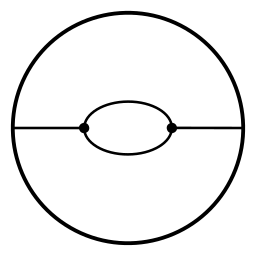
\includegraphics[width=0.1\textwidth, valign=c]{graphics/jacobi_bivalent_bubble.pdf}.
	\]
	Taking another copy \([\cdot, \cdot]'\) of the bracket tensor, one way to compute \(W_{\mathfrak{sl}_{2}} \left( J \right)\) is to let \([\cdot,\cdot]\) take the left trivalent vertex, and associate the upward facing half-edge to the first component. Let \([\cdot,\cdot]'\) take the right trivalent vertex and associate the downward facing half-edge to the first component. The cyclic orders determine the rest. Then the computation is to take the contraction of \([\cdot,\cdot]\) along components 1 and 3 with \([\cdot,\cdot]'\) along components 3 and 1. This gives
	\[2 h^{\ast} \otimes h^{\ast} + e^{\ast} \otimes f^{\ast} + f^{\ast} \otimes e^{\ast},\]
	and contracting along each component with a casimir to make them contravariant,
	\[
		T_{\mathfrak{sl}_{2}}
		\left(
		J
		\right)
		=
		\frac{1}{2} h \otimes h + e \otimes f + f \otimes e.
	\]
	Projecting this into \(\mathcal{U}(\mathfrak{g})\) and writing it in the PBW-basis,
	\[W_{\mathfrak{sl}_{2}}(J) = \frac{1}{2} h \otimes h - h + 2 e \otimes f.\]

	Finally, if we use the adjoint representation \(\operatorname{ad}\),
	\[
		\operatorname{ad}(h) =
		\begin{bmatrix}
			1 & 0 \\
			0 & -1
		\end{bmatrix}\;,\quad
		\operatorname{ad}(e) =
		\begin{bmatrix}
			0 & 1 \\
			0 & 0
		\end{bmatrix}\;,\quad
		\operatorname{ad}(f) =
		\begin{bmatrix}
			0 & 0 \\
			1 & 0
		\end{bmatrix}\;,\quad
	\]
	we get
	\[W_{\mathfrak{sl}_{2}, \operatorname{ad}}(J) = 3.\]
\end{example}

\begin{theorem}
	In Construction \ref{cons:lie-algebra-weight-system}, \(W_{\mathfrak{g}}\) is a well-defined \(\mathcal{U}(\mathfrak{g})\)-valued weight system, and \(W_{\mathfrak{g}, \rho}\) is a well-defined \(\mathbb{Q}\)-valued weight system.
\end{theorem}
%TODO (Zsuzsi) A picture to illustrate this construction is depreately needed. I understand what you're saying, but only because I know it.

\begin{proof}[\cite{on-the-vassiliev-knot-invariants}]
	To prove that \(W_{\mathfrak{g}, \rho}\) is well-defined, there are two points to prove. Jacobi diagrams are defined up to certain internal relations, namely \ref{eq:IHX} and \ref{eq:AS}, so the first point is that \(T_{\mathfrak{g}}(J)\) is invariant under \ref{eq:IHX} and \ref{eq:AS}. For \ref{eq:AS}, it follows from the antisymmetry of \([\cdot, \cdot]\), and for \ref{eq:IHX} it follows from the Jacobi relation. Alternatively, it follows from the second point as \ref{eq:IHX} and \ref{eq:AS} are consequences of \ref{eq:STU}.

	The second thing to prove is that \(W_{\mathfrak{g}}(J)\) is invariant under \ref{eq:STU}.
	If two chord diagrams differ by \ref{eq:STU}, on some univalent vertices associated with adjacent tensor factors \(y\) and \(x\), the construction gives
	\[\cdots \otimes [x, y]_{\mathfrak{g}} \otimes \cdots \qquad \text{and} \qquad (\cdots \otimes x \otimes y \otimes \cdots) - (\cdots \otimes y \otimes x \otimes \cdots),\]
	but this equality is exactly the defining relation of \(\mathcal{U}(\mathfrak{g})\).

	We come to the third point. There was one other arbitrary choice we made. The cyclic order of the univalent vertices of \(J\) induce a cyclic order on the components of the components of the tensor \(T_{\mathfrak{g}} \in \mathfrak{g}^{\otimes u}\). However, in the construction, a linear order which respects that cyclic order was chosen. We must show that any choice of linear order respecting the cyclic order produces the same result. This is no problem for the well-definition of \(W_{\mathfrak{g}, \rho}(J) = \operatorname{tr}(\rho(W_{\mathfrak{g}}(J)))\), as the trace is invariant under cyclic permutation. However for \(W_{\mathfrak{g}}(J) = [T_{\mathfrak{g}}(J)] \in \mathcal{U}(\mathfrak{g})\) it remains to prove cyclic permutation invariance. In fact a stronger statement is true. The diagram \(J\) itself is invariant under a cyclic permutation by Proposition \ref{prop:linear-jacobi-diagrams-cyclically-invariant}, so of course this is true for \(W_{\mathfrak{g}}(J)\).
\end{proof}

Let's look at a specific weight system for the Lie algebra \(\mathfrak{sl}_{2}\) \cite{on-the-vassiliev-knot-invariants, remarks-on-the-vassiliev-knot-invariants-coming-from-sl2}.
\begin{example}[Weight system for \({\mathfrak{sl}_{2}}\)]
	We use the metric Lie algebra from Example \ref{ex:simple-sl2-computation}. In \cite{remarks-on-the-vassiliev-knot-invariants-coming-from-sl2}, the following skein relation is derived:
	% NOTE: We are using the trace in the fundamental representation as our invariant bilinear form. If instead, we used the trace in the adjoint representation, we would get coefficients 1 instead of 4.
	\[
		W_{\mathfrak{sl}_{2}}
			\includegraphics[width=0.115\textwidth, valign=c]{graphics/sl2_skein_relation_h.pdf}
		=
		2 W_{\mathfrak{sl}_{2}}
			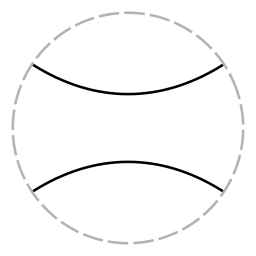
\includegraphics[width=0.115\textwidth, valign=c]{graphics/sl2_skein_relation_uu.pdf}
		-
		2 W_{\mathfrak{sl}_{2}}
			\includegraphics[width=0.115\textwidth, valign=c]{graphics/sl2_skein_relation_x.pdf}
	\]

	\begin{proof}
		Compute both sides by contracting and permuting tensors for the bracket, and casimir/metric in \(\mathfrak{sl}_{2}\). Both give
		\begin{align*}
			{}-h\otimes e\otimes h\otimes f+h\otimes e\otimes f\otimes h-h\otimes f\otimes h\otimes e+h\otimes f\otimes e\otimes h \\
			{}+e\otimes h\otimes h\otimes f-e\otimes h\otimes f\otimes h + 2 e\otimes f\otimes e\otimes f -2 e\otimes f\otimes f\otimes e \\
			{}+f\otimes h\otimes h\otimes e -f\otimes h\otimes e\otimes h -2 f\otimes e\otimes e\otimes f + 2 f\otimes e\otimes f\otimes e.
		\end{align*}
	\end{proof}

	\begin{shaded}
		In fact, this skein relation is an analogue of the vector triple product rule for the cross product in \(\mathbb{R}^{3}\), which is related to the Lie algebra \(\mathfrak{sl}_{2}\) \cite{introduction-to-vassiliev-invariants}. It has been further studied in \cite{riordan-trees-and-the-homotopy-sl2-weight-system}. There is also a cross product in \(\mathbb{R}^{7}\), related to the exceptional Lie algebra \(\mathfrak{g}_{2}\). However it does not obey the vector triple product rule.
	\end{shaded}

	\begin{remark}
		When computing via the \(\mathfrak{sl}_{2}\) skein relation above, it's possible to create a ``bubble'' (part of a diagram without any trivalent vertices). Since we are computing via contractions in the tensor algebra, this is to be interpreted as the contraction of the metric with the casimir. In a finite-dimensional Lie algebra, this is just the dimension, so for \(\mathfrak{sl}_{2}\), the factor \(3\).
		% TODO: Name drop the casimir above so they know what it is. (Zsuzsi) - Agreed.
        %TODO (Zsuzsi) An example picture?
	\end{remark}
\end{example}
\begin{question}
	Are there similar skein relations that the weight systems for the exceptional Lie algebras obey?
\end{question}

Bar-Natan's construction yields a way of extracting some information from \(\mathcal{A}\) by plugging in a metric Lie algebra -- doing so constructs some quotient of \(\mathcal{A}\). This naturally begs the question whether every all
%TODO (Zsuzsi) grammar
the information in \(\mathcal{A}\) can be extracted with some metric Lie algebra.

Computer enumeration of chord diagrams \cite{on-the-vassiliev-knot-invariants} prove this for order \(m \leq 9\), the order to which the dimensions \(\operatorname{dim}\mathcal{A}_{m} = \operatorname{dim}\mathcal{W}_{m}\) were known:
\[
	% TODO: Check that these are definitely the unframed numbers.
	\begin{tblr}{hlines, vlines}
		m									& 0 & 1 & 2 & 3 & 4 & 5  & 6  & 7  & 8  & 9   \\ \hline % & 10  & 11  & 12  \\
		\operatorname{dim}\mathcal{A}_{m}					& 1 & 1 & 2 & 3 & 6 & 10 & 19 & 33 & 60 & 104 \\ % & 184 & 316 & 548 \\
		\operatorname{dim}(\operatorname{span}(W_{\mathfrak{sl}_{n}, \mathfrak{gl}_{n}}))	& 1 & 1 & 2 & 3 & 6 & 10 & 19 & 33 & 60 & 104 \\
	\end{tblr}
\]
Here \(\operatorname{span}(W_{\{\mathfrak{g}, \rho\}})\) %but this is not the notation in the table, there you have $W$ with two lie algebras in the subscript, no reps
denotes the dimension of the subspace of \(\mathcal{W}_{m}\) spanned by weight systems coming from Costruction \ref{cons:lie-algebra-weight-system} on representations of classical Lie algebras \(\mathfrak{sl}_{n}\) and \(\mathfrak{gl}_{n}\).

\begin{conjecture}[Bar-Natan]
	\label{conj:lie-algebra-weight-systems-span}
	All weight systems are obtained as Lie algebra weight systems. In other words the set \(\{W_{\mathfrak{g}, \rho} \,|\, \text{\(\mathfrak{g}\) a Lie algebra}, \text{\(\rho\) a representation of \(\mathfrak{g}\)}\}\) spans \(\mathcal{W}\).
    %TODO (Zsuzsi) Now we have a rep, but no curly brackets
\end{conjecture}

Indeed the Lie action relation \(\rho([x, y]) = \rho(x)\rho(y) - \rho(y)\rho(x)\) as it was drawn graphically looks exactly like the \ref{eq:STU} relation in \(\mathcal{A}\). However, looks can be decieving and quite surprisingly this conjecture is false. The counterexample was found by Pierre Vogel \cite{algebraic-structures-on-modules-of-diagrams-preprint} in an attempt to answer the following related question:
\begin{question}[Vogel]
	\label{ques:vogel-universal-lie-algebra}
	Is there some single universal Lie algebra object whose weight system spans \(W_{\text{Lie}}\), the span of all Lie-algebraic weight systems?
\end{question}

We will look at examples of more general weight systems in Section~\ref{sec:non-lie-algebraic-weight-systems}. %TODO (ZSuzsi) I think this sentence is not needed: the title of 2.3 flows on beautifully from the Vogel question


\section{Non-Lie algebraic weight systems}
\label{sec:non-lie-algebraic-weight-systems}

Conjecture \ref{conj:lie-algebra-weight-systems-span} being false implies that \ref{eq:STU} is more general than \(\rho([x, y]) = \rho(x)\rho(y) - \rho(y)\rho(x)\). The same is true for \ref{eq:IHX} and \ref{eq:AS} compared to their strictly Lie-theoretic counterparts.
In fact, Construction \ref{cons:lie-algebra-weight-system} is just one example of a more general construction introduced by Vogel and Vaintrob to construct weight systems coming from metric Lie super-algebras.

The most general type of objects these constructions apply to are called by Vaintrob \cite{vassiliev-knot-invariants-and-lie-s-algebras} `Lie \(S\)-algebras', but we will follow the more modern approach of \cite{on-the-rozansky-witten-weight-systems, rozansky-witten-theory} and they will be known as Lie algebra objects in a symmetric monoidal category.

\begin{definition}
	A (\textbf{weak}) \textbf{monoidal category} is a category \(\mathcal{C}\) equipped with a functor
	\[
		\begin{array}{rccc}
			\otimes:	&\mathcal{C} \times \mathcal{C}		&\longrightarrow	&\mathcal{C}\\
					&(A, B)					&\longmapsto		&A \otimes B,
		\end{array}
	\]
	a \textbf{unit} object \(k \in \mathcal{C}\), and natural isomorphisms
	\[
		 \otimes \circ (\otimes \times \operatorname{id}) \longrightarrow \otimes \circ (\operatorname{id} \times \otimes)  \quad \text{ and }\ \quad  \otimes \longrightarrow \operatorname{id}
	\]
	satisfying some relations known as the pentagon and triangle relations.
    %TODO (Zsuzsi) state the relations, or at the very least, reference them
    The natural isomorphisms give isomorphisms
	\[(A \otimes B) \otimes C \cong A \otimes (B \otimes C), \qquad k \otimes A \cong A \cong A \otimes k\]
	for every tuple of objects \(A, B\) and \(C\) in \(\mathcal{C}\). If these isomorphisms are equalities, then \(\mathcal{C}\) is a \textbf{strict} monoidal category.
\end{definition}

\begin{remark}
	\label{rem:coherence-for-monoidal-categories}
	Omitting the details, we assume that these natural isomorphisms are equalities, for example that \((A \otimes B) \otimes C = A \otimes (B \otimes C)\). This is acceptable by the coherence theorem for monoidal categories which says that every monoidal category is equivalent to a strict monoidal category, and it's why we omit the pentagon and triangle relations in the definition above. We refer to \cite{higher-operads-higher-categories} for details. %TODO (Zsuzsi) This is a big black box, which is justified but the reference should be more specific than a whole book.
\end{remark}

\begin{definitions}
	\begin{enumerate}
		\item The \textbf{flip functor} is the functor
			\[
				\begin{array}{rccc}
					\sigma:		&\mathcal{C} \times \mathcal{C}		&\longrightarrow	&\mathcal{C} \times \mathcal{C}\\
						&(A, B)					&\longmapsto		&(B, A).
				\end{array}
			\]

		\item A \textbf{symmetric monoidal category} is a monoidal category \(\mathcal{C}\) equipped with a \textbf{symmetry natural isomorphism} \(\tau\)
			\[\otimes \longrightarrow \otimes \circ \sigma\]
			satisfying the hexagon relation. The \textbf{hexagon relation} is the relation that the isomorphisms
			\[
				\tau_{A, B}: A \otimes B \overset{\cong}{\longrightarrow} B \otimes A
			\]
			coming from the natural isomorphism \(\tau\) obey
			\[\tau_{A, B \otimes C} = (\operatorname{id}_{B} \mathbin{\otimes} \tau_{A, C}) \circ (\tau_{A, B} \mathbin{\otimes} \operatorname{id}_{C})\]
			for every pair of objects \(A\), and \(B\) in \(\mathcal{C}\). 
	\end{enumerate}
\end{definitions}
The hexagon relations have six terms instead of three when the associators omitted due to Remark \ref{rem:coherence-for-monoidal-categories} are reintroduced. %TODO (Zsuzsi) You hadn't used the word associator before, someone who doesn't already know this wouldn't understand

If the tensor %TODO (zsuzsi) monoidal?
category \(\mathcal{C}\) is additionally additive, we can define the following. %TODO (Zsuzsi) "we define lie algebra objects in \(\mathcal{C}\) "

\begin{definitions}
	\begin{enumerate}
		\item A \textbf{Lie algebra object} in an additive symmetric tensor category \(\mathcal{C}\) is an object \(L\) equipped with a bracket morphism \(\beta\) 
        %TODO (Zsuzsi) Domain and codomain of $\beta$?
        such that
			\[\left( \beta \circ (\beta \otimes \operatorname{id}) \right) \circ (1 + \tau_{123} + (\tau_{123})^{2}) = 0 \qquad \text{and} \qquad \beta + \beta \circ \tau = 0.\]
			Graphically, in terms of the string diagrams of the previous section, this is
			\[
				\def\svgscale{0.31}
				\adjustbox{valign=c}{\input{graphics/jacobi_symmetric_arbitrary_monoidal_cat_xyz.pdf_tex}}
				\quad
				+
				\quad
				\def\svgscale{0.31}
				\adjustbox{valign=c}{\input{graphics/jacobi_symmetric_arbitrary_monoidal_cat_yzx.pdf_tex}}
				\quad
				+
				\quad
				\def\svgscale{0.31}
				\adjustbox{valign=c}{\input{graphics/jacobi_symmetric_arbitrary_monoidal_cat_zxy.pdf_tex}}
				\quad
				=
				\quad
				0,
			\]
			\[
				\def\svgscale{0.35}
				\adjustbox{valign=c}{\input{graphics/bracket_antisymmetry_arb_mon_cat_id.pdf_tex}}
				\quad
				+
				\quad
				\def\svgscale{0.35}
				\adjustbox{valign=c}{\input{graphics/bracket_antisymmetry_arb_mon_cat_swap.pdf_tex}}
				\quad
				=
				\quad
				0.
			\]
    %TODO (Zsuzsi) Declare that the dot is beta?
		\item A \textbf{representation of a Lie algebra object} \(L\) in \(\mathcal{C}\) into an object \(V\) in \(\mathcal{C}\) is a morphism \(\rho: L \otimes V \to V\), such that
			\[
				\def\svgscale{0.31}
				\adjustbox{valign=c}{\input{graphics/string_diagram_lie_action_arb_mon_cat_s.pdf_tex}}
				\quad
				=
				\quad
				\def\svgscale{0.31}
				\adjustbox{valign=c}{\input{graphics/string_diagram_lie_action_arb_mon_cat_t.pdf_tex}}
				\quad
				-
				\quad
				\def\svgscale{0.31}
				\adjustbox{valign=c}{\input{graphics/string_diagram_lie_action_arb_mon_cat_u.pdf_tex}}
				.
			\]
            %TODO (Zsuzsi) Again, explain the notation that $V$ is the thick line and $\rho$ is the trivalent vertex with two thick and one thin edges
		\item A \textbf{metric Lie algebra object} \(L\) in \(\mathcal{C}\) is a Lie algebra object in \(\mathcal{C}\), further equipped with the following modules over \(L\)...
        %TODO (Zsuzsi) Incomplete?
	\end{enumerate}
\end{definitions}


We will give various concrete examples of Lie algebra objects in different symmetric tensor categories later. But for now, let's show that this data can still be used to construct weight systems, generalising Construction \ref{cons:lie-algebra-weight-system}.

\begin{theorem}[\cite{ vassiliev-knot-invariants-and-lie-s-algebras}]
	% TODO: Check that all the ajectives have been defined, or at least thought about.
	Let \(\mathcal{C}\) be a rigid, additive, symmetric monoidal category, \(L\) a metric Lie algebra in \(\mathcal{C}\), and \(M\) a dualisable representation \(\eta\). 
    %TODO (Zsuzsi) is $M$ the representation, or $\eta$?
    Then, there is a weight system
	\[W_{L, \eta}: \mathcal{A} \longrightarrow \mathcal{C}(k, k) \cong k.\]
\end{theorem}
\begin{proof}
	Similar to the proof of the construction... %TODO (Zsuzsi) Incomplete?
\end{proof}

The difference between this construction and Bar-Natan's original one is the treatment of the symmetry natural isomorphism \(\tau\). This tells us which isomorphism to use when rearranging the tensor factors. The most obvious isomorphism would be the identity, as it was in the original construction, corresponding to when \(\mathcal{C}\) is a strict symmetric (strict) monoidal category. However unlike for general monoidal categories, not every symmetric monoidal category is equivalent to a strict symmetric monoidal category. 
%TODO (Zsuzsi) So maybe pentagon, triangle and true hexagon should be stated above?
At a down-to-earth level, Lie algebra objects with non-trivial symmetry isomorphisms are necessary to pick up all the structure in \(\mathcal{A}\).

\begin{example}
	If we take \(\mathcal{C} = \mathbf{sVect}\), the symmetric monoidal category of super vector spaces, the Lie algebra objects are the following.

	A \textbf{Lie superalgebra} \(\mathfrak{g}\) is a vector space with a \(\mathbb{Z} / 2\mathbb{Z}\) grading, equipped with a bracket \([\cdot,\cdot]: \mathfrak{g} \otimes \mathfrak{g} \to \mathfrak{g}\) satisfying some axioms to follow. The grading induces the splitting \(\mathfrak{g} = \mathfrak{g}_{0} \oplus \mathfrak{g}_{1}\), and the direct summand \(\mathfrak{g}_{0}\) is known as the \textbf{even} part and the summand \(\mathfrak{g}_{1}\) is known as the \textbf{odd} part.

	The axioms a Lie superalgebra must satisfy are the following analogues of the usual lie algebra axioms. Let \(x, y, z\) be homogeneous elements, so in \(\mathfrak{g}_{i}, \mathfrak{g}_{j}\), and \(\mathfrak{g}_{k}\) respectively, then \textbf{super symmetry} axiom is
		\[[x, y] = - (-1)^{ij}[y, x],\]
		and the \textbf{super Jacobi identity} is the axiom
		\[(-1)^{ik}[x, [y, z]] + (-1)^{ji}[y, [z, x]] + (-1)^{kj}[z, [x, y]] = 0.\]
\end{example}

Shortly after Conjecture \ref{conj:lie-algebra-weight-systems-span} was made, the following results were achieved based on constructions with the exceptional Lie superalgebra \(\mathfrak{D}(2, 1; \alpha)\).

\begin{theorem}
	There are primitive Jacobi diagrams of order at least 17 \cite{algebraic-structures-on-modules-of-diagrams-preprint} and at least 15 \cite{on-vassiliev-invariants-not-coming-from-semisimple-lie-algebras} which vanish under all Lie algebra weight systems. 
\end{theorem}

Furthermore, as was known about shortly after but not published until significantly later,
\begin{theorem}
Vogel's diagram of order 17 vanishes also on all Lie superalgebra weight systems \cite{algebraic-structures-on-modules-of-diagrams}.
\end{theorem}

\begin{corollary}
	The set of Lie (super)algebra weight systems does not span \(\mathcal{W}\).
\end{corollary}

In general, it is still unknown to what exact level of generality one needs to go (what type of symmetric monoidal categories need to be considered) in order to generate all weight systems. We hereby provide a succinct review the current state of the literature on the subject.

Roberts and Willerton in \cite{rozansky-witten-theory} and \cite{on-the-rozansky-witten-weight-systems} examine weight systems constructructed from Lie algebra objects in the derived category of complex manifolds. Such weight systems are candidates for being able to detect knot orientation, which Lie algebra weight systems cannot \cite{on-the-vassiliev-knot-invariants}. However, computing these weight systems is difficult, and to our knowledge, no computations exist in the literature.

More recently Aizawa-Kimura \cite{universal-weight-systems-from-a-mimimal-Z22-graded-lie-algebra}, have conducted some preliminary investigations into the class of colour Lie algebras (also known as \(\epsilon\)-Lie algebras). This class generalises the \(\mathbb{Z}/2\mathbb{Z}\) grading on Lie superalgebras to a more general type of group and sign rule. The example they present lies within the span of the \(\mathfrak{sl}_{2}\) and \(\mathfrak{gl}_{1 | 1}\) weight systems.


\section{Some weight systems at the exceptional Lie algebras}
\label{sec:some-weight-systems-at-the-exceptional-lie-algebras}

The original motivation for the work of Vogel \cite{algebraic-structures-on-modules-of-diagrams-preprint, algebraic-structures-on-modules-of-diagrams} and written more explicity in \cite{vassiliev-theory-and-the-universal-lie-algebra} was to construct a universal object generalising all simple Lie algebras, whose weight systems span \(\mathcal{W}\). \textbf{Insert a summary of the Vogel universality story.} %TODO (Zsuzsi) Don't forget...

The relation for \(W_{\mathfrak{sl}_{2}}\) given above is entirely internal to the lie algebra; it doesn't involve projecting to the universal enveloping algebra or choosing a representation. In terms of Vogel universality, this is known as `lying in the adjoint sector'.

Present implicitly in \cite{algebraic-structures-on-modules-of-diagrams} is a way to determine, local relations internal to any simple lie algebra in terms of its parameters \(\alpha, \beta\) and \(\gamma\), and some complicated `marked' elements of \(\mathcal{A}\) defined recursively. These were written out explicitly in the recent preprint \cite[Appendix]{construction-of-lie-algebra-weight-system-kernel-via-vogel-algebra}. The use of different normalisations of the parameters \(\alpha, \beta\) and \(\gamma\) 
%TODO (Zsuzsi) What are paramenters?
in these two sources makes computing explicit relations tedious. Furthermore, the relations are general enough to hold for any Lie superalgebra, but can be simplified in the specific case of a Lie algebra.

Theorem 6.3(2) of \cite{algebraic-structures-on-modules-of-diagrams} gives a relation in \(W_{\mathfrak{g}_{2}}\).
\[
	\begin{array}{ll}
		-6
		W_{\mathfrak{g}_{2}}
		\includegraphics[width=0.115\textwidth, valign=c]{graphics/local_jacobi_w4_column.pdf}
		-
		12
		W_{\mathfrak{g}_{2}}
		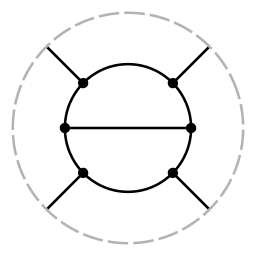
\includegraphics[width=0.115\textwidth, valign=c]{graphics/local_jacobi_w4_crossbeam.pdf}
		+
		18
		W_{\mathfrak{g}_{2}}
		\includegraphics[width=0.115\textwidth, valign=c]{graphics/local_jacobi_tw4.pdf} \\
		\quad
		{}+\displaystyle\frac{7}{4}
		W_{\mathfrak{g}_{2}}
		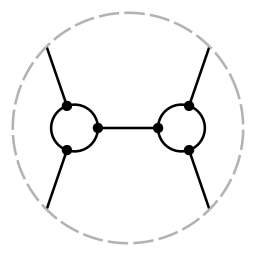
\includegraphics[width=0.115\textwidth, valign=c]{graphics/local_jacobi_tth.pdf}
		+
		20
		W_{\mathfrak{g}_{2}}
		\includegraphics[width=0.115\textwidth, valign=c]{graphics/local_jacobi_smooth.pdf}
		+
		20
		W_{\mathfrak{g}_{2}}
		\includegraphics[width=0.115\textwidth, valign=c]{graphics/local_jacobi_cross.pdf}
		& =
		\,\,\,
		0
	\end{array}
\]
However, by some well-known identies internal to Jabobi diagrams, these diagrams can be simplified.
\begin{lemma}
	\label{lem:tribubble-is-half-bibubble}
	In \(\mathcal{A}\) the `trivalent-bubble' vertex is proprtional to the regular trivalent vertex with a bivalent bubble inserted on any one of the half-edges.
	\[
		\includegraphics[width=0.115\textwidth, valign=c]{graphics/local_jacobi_triangle.pdf}
		=
		\frac{1}{2}
		\includegraphics[width=0.115\textwidth, valign=c]{graphics/local_jacobi_triangle_bubbled.pdf}
	\]
\end{lemma}
\begin{proof}
	Apply \ref{eq:IHX} to any pair of vertices, then three applications of \ref{eq:AS}.
	\[
		\includegraphics[width=0.115\textwidth, valign=c]{graphics/local_jacobi_triangle.pdf}
		=
		\includegraphics[width=0.115\textwidth, valign=c]{graphics/local_jacobi_triangle_is_bubble_h.pdf}
		+
		\includegraphics[width=0.115\textwidth, valign=c]{graphics/local_jacobi_triangle_is_bubble_x.pdf}
		=
		\includegraphics[width=0.115\textwidth, valign=c]{graphics/local_jacobi_triangle_bubbled.pdf}
		-
		\includegraphics[width=0.115\textwidth, valign=c]{graphics/local_jacobi_triangle.pdf}
	\]
\end{proof}
\begin{lemma}
	\label{lem:bibubble-proportional-to-line}
	In Lie algebraic weight systems, the bubble is proportional to the line.
	\[
		W_{\mathfrak{g}}
		\includegraphics[width=0.115\textwidth, valign=c]{graphics/local_jacobi_bivalent_bubble.pdf}
		=
		\lambda
		W_{\mathfrak{g}}
		\includegraphics[width=0.115\textwidth, valign=c]{graphics/local_jacobi_line.pdf}
	\]
\end{lemma}
\begin{proof}
	\begin{shaded}
		It's in CDM but it's unsatisfying. If it can be proved for Lie algebras it should be able to be proved in a way where it's obvious it doesn't work for Lie superalgebras, with without referring to the dual basis and its properties.
	\end{shaded}
\end{proof}

Simplifying Vogel's relation via these lemmas (we use the metric in which \(\lambda = 1/4\)), gives the following relation. 
%TODO (Zsuzsi) Explain above that $\lambda$ depends on the metric?

\begin{proposition}
	\[
		\begin{array}{ll}
			-6
			W_{\mathfrak{g}_{2}}
			\includegraphics[width=0.115\textwidth, valign=c]{graphics/local_jacobi_w4_column.pdf}
			-
			12
			W_{\mathfrak{g}_{2}}
			\includegraphics[width=0.115\textwidth, valign=c]{graphics/local_jacobi_w4_crossbeam.pdf}
			+
			36
			W_{\mathfrak{g}_{2}}
			\includegraphics[width=0.115\textwidth, valign=c]{graphics/local_jacobi_w4.pdf} \\
			\quad \quad
			{}+
			7
			W_{\mathfrak{g}_{2}}
			\includegraphics[width=0.115\textwidth, valign=c]{graphics/local_jacobi_h.pdf}
			+
			20
			W_{\mathfrak{g}_{2}}
			\includegraphics[width=0.115\textwidth, valign=c]{graphics/local_jacobi_smooth.pdf}
			-
			20
			W_{\mathfrak{g}_{2}}
			\includegraphics[width=0.115\textwidth, valign=c]{graphics/local_jacobi_cross.pdf}
		& =
		\,\,\,
		0
		\end{array}
	\]
\end{proposition}

This relation is true for any diagram into which each term is inserted. In-particular, it remains true after rotating all terms a quarter rotation clockwise. However it's not obvious that this is true,
%TODO (Zsuzsi) It *is* obvious though that this is true... I guess it's just not obvious how to use relations to equate the two?
 and various other relations have to be applied to turn the rotated version into the original relation. This suggests that perhaps the relation is a consequence of a similar relation.

\begin{theorem}
	\label{thm:g2-unboxing-relation}
	In the algebra \(\mathfrak{g}_{2}\), the weight systems obey
	\[
		\begin{array}{lll}
			W_{\mathfrak{g}_{2}}
			\includegraphics[width=0.115\textwidth, valign=c]{graphics/local_jacobi_w4.pdf}
			& = &
			\displaystyle\frac{2}{3}
			W_{\mathfrak{g}_{2}}
			\includegraphics[width=0.115\textwidth, valign=c]{graphics/local_jacobi_h.pdf}
			+
			\displaystyle\frac{2}{3}
			W_{\mathfrak{g}_{2}}
			\includegraphics[width=0.115\textwidth, valign=c]{graphics/local_jacobi_i.pdf}
			\\
			&& \quad +
			\displaystyle\frac{5}{6}
			W_{\mathfrak{g}_{2}}
			\includegraphics[width=0.115\textwidth, valign=c]{graphics/local_jacobi_smooth.pdf}
			+
			\displaystyle\frac{5}{6}
			W_{\mathfrak{g}_{2}}
			\includegraphics[width=0.115\textwidth, valign=c]{graphics/local_jacobi_smooth_vert.pdf}
			+
			\displaystyle\frac{5}{6}
			W_{\mathfrak{g}_{2}}
			\includegraphics[width=0.115\textwidth, valign=c]{graphics/local_jacobi_cross.pdf}.
		\end{array}
	\]
\end{theorem}

\begin{proof}
	Compute the tensors corresponding to both sides.
\end{proof}

This is an analogue of a relation for \(\mathfrak{sl}_{3}\) found by Yoshizumi and Kuga in \cite{some-formulas-in-sl3-weight-systems}. This was used recently by Yang in \cite{on-values-of-sl3-weight-system-on-chord-diagrams-whose-intersection-graph-is-complete-bipartite} to compute the value of the \(\mathfrak{sl}_{3}\) weight systems on the following infinite sequence of chord diagrams.

\begin{definition}
	The \(i\)th \textbf{bookshelf diagram}, \(B_{i}\), is the Jacobi diagram
	\[
		\def\svgscale{0.25}
		\raisebox{-20pt}{\input{graphics/jacobi_bookshelf.pdf_tex}}
	\]
\end{definition}

In \cite{on-values-of-sl3-weight-system-on-chord-diagrams-whose-intersection-graph-is-complete-bipartite}, a third-order recursion relation for the values of the \(\mathfrak{sl}_{3}\) weight system on the bookshelf diagrams is found. We use the same idea with the new relation of Theorem \ref{thm:g2-unboxing-relation} to compute their values under the \(\mathfrak{g}_{2}\) weight system.

\begin{theorem}
	% TODO: Define the casimir element somewhere, probably above.
	The values of the bookshelf diagram \(B_{i}\) are at most quadratic in the (quadratic) casimir element \(c\) of \(\mathfrak{g}_{2}\). In particular,
	\[W_{\mathfrak{g}_{2}}(B_{i}) = c^{2} \left( \frac{1}{14} 4^{n} + \frac{27}{112} (5/3)^{n} + \frac{11}{16} (-1)^{n} \right) + c\left( 2^{n} + \frac{8}{3} (5/3)^{n} -\frac{11}{8}(-1)^{n} \right).\]
\end{theorem}

\begin{proof}
	Apply Theorem \ref{thm:g2-unboxing-relation}, to the rightmost box on a bookshelf diagram.
	\[
		\begin{array}{lll}
			W_{\mathfrak{g}_{2}}
			\def\svgscale{0.25}
			\raisebox{-29pt}{\input{graphics/jacobi_bookshelf.pdf_tex}}
			& = &
			\displaystyle\frac{2}{3}
			W_{\mathfrak{g}_{2}}
			\def\svgscale{0.25}
			\raisebox{-29pt}{\input{graphics/jacobi_bookshelf_h.pdf_tex}}
			+
			\displaystyle\frac{2}{3}
			W_{\mathfrak{g}_{2}}
			\def\svgscale{0.25}
			\raisebox{-29pt}{\input{graphics/jacobi_bookshelf_i.pdf_tex}} \\
			&& +
			\displaystyle\frac{5}{6}
			W_{\mathfrak{g}_{2}}
			\def\svgscale{0.25}
			\raisebox{-29pt}{\input{graphics/jacobi_bookshelf_horisontalsmoothing.pdf_tex}}
			+
			\displaystyle\frac{5}{6}
			W_{\mathfrak{g}_{2}}
			\def\svgscale{0.25}
			\raisebox{-29pt}{\input{graphics/jacobi_bookshelf_verticalsmoothing.pdf_tex}}
			+
			\displaystyle\frac{5}{6}
			W_{\mathfrak{g}_{2}}
			\def\svgscale{0.25}
			\raisebox{-29pt}{\input{graphics/jacobi_bookshelf_diagonalsmoothing.pdf_tex}}
		\end{array}
	\]

	Applying \ref{eq:STU} to the final term gives
	\[
		W_{\mathfrak{g}_{2}}
		\def\svgscale{0.25}
		\raisebox{-29pt}{\input{graphics/jacobi_bookshelf_diagonalsmoothing.pdf_tex}}
		=
		W_{\mathfrak{g}_{2}}
		\def\svgscale{0.25}
		\raisebox{-29pt}{\input{graphics/jacobi_bookshelf_h.pdf_tex}}
		+
		W_{\mathfrak{g}_{2}}
		\def\svgscale{0.25}
		\raisebox{-29pt}{\input{graphics/jacobi_bookshelf_horisontalsmoothing.pdf_tex}}
	\]
	By Lemma \ref{lem:tribubble-is-half-bibubble}, we have
	\[
		W_{\mathfrak{g}_{2}}
		\def\svgscale{0.25}
		\raisebox{-29pt}{\input{graphics/jacobi_bookshelf_h.pdf_tex}}
		=
		2^{i - 2}
		W_{\mathfrak{g}_{2}}
		\def\svgscale{0.25}
		\raisebox{-29pt}{\input{graphics/jacobi_bookshelf_h_popped.pdf_tex}}
		=
		2^{i - 2} 4 c^{2}
	\]
	This calculation of the \(\mathfrak{g}_{2}\) weight system on this diagram first appears in the literature in the PhD thesis of A. Kaishev which we have been unable to source, however it also appears in \cite[p. 181]{introduction-to-vassiliev-invariants}. Our computer program also verifies it. By Lemma \ref{lem:bibubble-proportional-to-line},
	\[
		W_{\mathfrak{g}_{2}}
		\def\svgscale{0.25}
		\raisebox{-29pt}{\input{graphics/jacobi_bookshelf_verticalsmoothing.pdf_tex}}
		=
		4^{i - 2}
		W_{\mathfrak{g}_{2}}
		\def\svgscale{0.25}
		\raisebox{-29pt}{\input{graphics/jacobi_bookshelf_verticalsmoothing_popped.pdf_tex}}
		=
		4^{i - 2}c^{2}
	\]

	All in all,
	\[
		W_{\mathfrak{g}_{2}}
		\def\svgscale{0.25}
		\raisebox{-29pt}{\input{graphics/jacobi_bookshelf.pdf_tex}}
		=
		\displaystyle\frac{2}{3}
		W_{\mathfrak{g}_{2}}
		\def\svgscale{0.25}
		\raisebox{-29pt}{\input{graphics/jacobi_bookshelf_i.pdf_tex}}
		+
		\displaystyle\frac{5}{3}
		W_{\mathfrak{g}_{2}}
		\def\svgscale{0.25}
		\raisebox{-29pt}{\input{graphics/jacobi_bookshelf_horisontalsmoothing.pdf_tex}}
		+
		\frac{5}{6} 4^{i - 2} c^{2}
		+
		\frac{11}{6} 2^{i - 2} c
	\]
	so setting
	\[
		g_{i} =
		W_{\mathfrak{g}_{2}}
		\def\svgscale{0.25}
		\raisebox{-29pt}{\input{graphics/jacobi_bookshelf.pdf_tex}}
	\]
	we have the second-order non-homogeneous recursion relation for \(g_{i}\)
	\[g_{i + 2} = \frac{2}{3} g_{i + 1} + \frac{5}{3} g_{i} + \frac{5}{6} 4^{i} c^{2} + \frac{11}{6} 2^{i} c.\]
	Its fourth-order homogeneous form is
	\[g_{i + 4} - \frac{20}{3} g_{i + 3} + \frac{31}{3}g_{i + 2} + \frac{14}{3} g_{i + 1} - \frac{40}{3} g_{i} = 0.\]
	
	To solve this we need the inital conditions \(g_{1}, g_{2}\) and \(g_{3}\). The first two come from the same computations of Kaishev \cite[p. 181]{introduction-to-vassiliev-invariants}, whereas the third we have to compute ourselves.

	Computing in sagemath the tensor corresponding to the diagram
	\[
	\includegraphics[width=0.115\textwidth, valign=c]{graphics/local_jacobi_w4.pdf}
	\]
	then projecting it to \(\mathcal{U}(\mathfrak{g}_{2})\) gives the value, but expressed in the PBW basis rather than as a polynomial in the casimir. There are two generating casimirs of \(\mathfrak{g}_{2}\). 
    %Maybe talk about $g_3$ first, rather than the other one?
    The other is of degree \(6\), but \(g_{3}\) is a degree \(4\) element of \(Z(\mathfrak{g}_{2})\), so it will be a polynomial in \(c\) of degree two or less. Evaluating \(\rho(g_{3})\) with \(\rho\) being the trivial representation, the seven-dimensional standard representation, and the fourteen-dimensional adjoint representation gives the following values.
	\begin{align*}
		\rho_{\text{tr.}}(c) &= 0	& \rho_{\text{tr.}}(g_{3}) &= 0 \\
		\rho_{\text{st.}}(c) &= 2	& \rho_{\text{st.}}(g_{3}) &= \frac{380}{9} \\
		\rho_{\text{ad.}}(c) &= 4	& \rho_{\text{ad.}}(g_{3}) &= \frac{1120}{9}
	\end{align*}
	So by the Lagrange interpolation formula,
	\[g_{3} = 5c^{2} + \frac{100}{9}c.\]
	Solving the recurrence relation with these inital conditions yields the formula
	\[
	g_{i}
	=
	c^{2} \left( \frac{1}{14} 4^{i} + \frac{27}{112} (5/3)^{i} + \frac{11}{16} (-1)^{i} \right) + c\left( 2^{i} + \frac{8}{3} (5/3)^{i} -\frac{11}{8}(-1)^{i} \right).
	\]
\end{proof}

We use the same method to compute the a relation in the weight system \(W_{\mathfrak{g}}\) for the exceptional Lie algebra \(\mathfrak{g} = {\mathfrak{f}_{4}}\). 
%TODO (Zsuzsi) State as Theorem?
\[
	\begin{array}{ll}
		-12
		W_{\mathfrak{f}_{4}}
		\includegraphics[width=0.115\textwidth, valign=c]{graphics/local_jacobi_w4_column.pdf}
		-
		24
		W_{\mathfrak{f}_{4}}
		\includegraphics[width=0.115\textwidth, valign=c]{graphics/local_jacobi_w4_crossbeam.pdf}
		+
		54
		W_{\mathfrak{f}_{4}}
		\includegraphics[width=0.115\textwidth, valign=c]{graphics/local_jacobi_w4.pdf} \\
		\quad \quad
		{}-
		4
		W_{\mathfrak{f}_{4}}
		\includegraphics[width=0.115\textwidth, valign=c]{graphics/local_jacobi_h.pdf}
		+
		5
		W_{\mathfrak{f}_{4}}
		\includegraphics[width=0.115\textwidth, valign=c]{graphics/local_jacobi_smooth.pdf}
		-
		5
		W_{\mathfrak{f}_{4}}
		\includegraphics[width=0.115\textwidth, valign=c]{graphics/local_jacobi_cross.pdf}
		& =
		\,\,\,
		0.
	\end{array}
\]

The dimension of \(\mathfrak{g}_{2}\) is \(14\), and tensor contraction with sagemath takes about ten seconds on a [computer specs]. One the other hand, \(\operatorname{dim} \mathfrak{f}_{4} = 52\), and calculation takes several hours on [computer specs escona].%TODO(Zsuzsi) Don't forget to fill these in


Finally, we note that for \(\mathfrak{sl}_{4}\) the arguments given above do not work.

\begin{theorem}
	In the weight system corresponding to the Lie algebra \(\mathfrak{sl}_{4}\), there is no linear relation between the diagrams
	\[
		\includegraphics[width=0.115\textwidth, valign=c]{graphics/local_jacobi_w4.pdf},
		\includegraphics[width=0.115\textwidth, valign=c]{graphics/local_jacobi_h.pdf},
		\includegraphics[width=0.115\textwidth, valign=c]{graphics/local_jacobi_i.pdf},
		\includegraphics[width=0.115\textwidth, valign=c]{graphics/local_jacobi_smooth.pdf},
		\includegraphics[width=0.115\textwidth, valign=c]{graphics/local_jacobi_smooth_vert.pdf}
		\;\text{and}\;
		\includegraphics[width=0.115\textwidth, valign=c]{graphics/local_jacobi_cross.pdf}.
	\]
\end{theorem}

\begin{proof}
	By computer verification with sagemath, the span of the corresponding tensors in \((\mathfrak{sl}_{4})^{\otimes 4}\) is six-dimensional.
\end{proof}



\section{A universal metric Lie algebra object}
\label{sec:a-universal-metric-lie-algebra-object}

There is, however,  a theoretical construction of Hinnich-Vaintrob \cite{cyclic-operads-and-the-algebra-of-chord-diagrams}. They construct a Lie algebra object in a symmetric tensor category with  a ``weight system'' (in a certain sense) which is isomorphic to \(\mathcal{A}\). In Chapter \ref{ch:welded-knots-isometry-lie-algebras-and-arrow-diagrams}, we will examine an object, analagous to the space of welded knots, rather than knots.

Note, however that the objects in this category are not sets, but simply objects, so the result is useful theoretically rather than computationally.

Their construction uses the language of operads and props, which we review. For all of the below, we assume categories are linear.

Some operations on a set can always be composed by taking as input the output of another operation. These compositions alyways obey certain rules. If the set is a vector space, the operations too form a vector space. An operad captures this concept of operations on some object on a category abstractly.

\begin{definition}
	An \textbf{operad} \(\mathcal{O}\) in monoidal category \(\mathcal{C}\) consists of:

	\begin{itemize}
		\item a collection of objects in \(\mathcal{C}\), \(\{\mathcal{O}(n)\}_{n \in \mathbb{N}}\), with \(\mathcal{O}(n)\) known as the \textbf{\(n\)-ary operations}
		\item an element \(\id \in \mathcal{O}(1)\).
		\item an action of the symmetric group \(S_{n}\) on each \(\mathcal{O}(n)\)
		\item a series of composition morphisms: for each \(n\) and \(k_{1}, k_{2}, \cdots, k_{n} \in \mathbb{N}\)
			% TODO: Convert to array like above
			\begin{align*}
				\circ_{n}: \mathcal{O}(n) \otimes \mathcal{O}(k_{1}) \otimes \mathcal{O}(k_{2}) \otimes \cdots \otimes \mathcal{O}(k_{n}) &\longrightarrow \mathcal{O}(k_{1} + k_{2} + \cdots + k_{n}) \\
				\theta \otimes \theta_{1} \otimes \theta_{2} \otimes \cdots \otimes \theta_{n} &\longmapsto \theta \circ (\theta_{1} \otimes \theta_{2} \otimes \cdots \otimes \theta_{n})
			\end{align*}
	\end{itemize}
	satisfying the following axioms: [Do I want all of these??]
	\begin{itemize}
		\item Associativity --- but not of the operations, of composition of the operations
		\item Equivariance --- permuting the inputs of \(\theta\), permuting the morphisms input to \(\theta\), and inversely block-permuting their inputs does nothing.
		\item The action of the symmetric group agrees with its action in \(\mathcal{C}\).
	\end{itemize}
\end{definition}

\begin{definition}
	An \textbf{algebra \(A\) over the operad \(\mathcal{O}\) (in \(\mathcal{C}\))} is an object of \(\mathcal{C}\) satisfying certain natural compatibility conditions.
\end{definition}

In essence, an algebra over an operad is an object in \(\mathcal{C}\) whose operations obey the rules defined by \(\mathcal{O}\).

\begin{example}
	\begin{shaded}
		Nobody has ever showed me a definition of the Lie operad. I suppose it's just a quotient of the rooted binary trees operad. Also add an example of at least one other operad (maybe associative or commutative).
	\end{shaded}
\end{example}

Composition in operads is something like contraction in a symmetric monoidal category, but with restictions on what can be contracted: only outputs and inputs. From two operations, one can take their tensor product, but this doesn't fit into the notion of an operad, as it has two outputs.

A step towards allowing general contractions is to allow multiple outputs, thereby considering not just operations but, for example in \(\mathcal{C} = \mathbf{Vect}\), general multilinear functions. Operads were abstractions of the operations on some object (say, \(A\)), i.e. morphisms \(A^{\otimes n} \to A\). Props will be abstractions of all maps \(A^{\otimes n} \to A^{\otimes m}\).

\begin{definition}
	A \textbf{prop} is a symmetric monoidal category where every object is of the form \(A^{\otimes n}\) for some object \(A\).
\end{definition}

\begin{definition}
	An \textbf{algebra \(A\) over the prop \(\mathbf{P}\) (in \(\mathcal{C}\))} is tensor functor \(\alpha: \mathbf{P} \to \mathcal{C}\).
\end{definition}

\begin{shaded}
	Since this is a tensor-functor from a tensor category generated by a single object, this is equivalent to a choice of object in \(\mathcal{C}\) such that [...figure out what...].

	\begin{remark}
		There is an adjunction \(\mathsf{Prop} \to \mathsf{Oper}\). The operad to prop direction looks at all the morphisms \((n \to 1)\) in the prop, the other direction takes arbitrary tensor products of things in the operad.
	\end{remark}
\end{shaded}

\begin{proposition}
	The notions of algebra over a prop and algebra over an operad are equivalent. \(A \in \mathcal{C}\) is an algebra over the operad \(\mathcal{O}\) if and only if it is an algebra over the prop \(\mathbf{P}(\mathcal{O})\).
\end{proposition}

Now the only difference between contraction and what is governed by our prop is the inputs vs outputs. Remember the action of the symmetric group comes from the symmetry of the symmetric monoidal category \(\mathcal{C}\). But this only permutes inputs and outputs among themselves. We want a way to permute inputs with outputs. This cannot actually be done in an operad, but if the operad is of a certain kind, the same effect can be achieved in terms of how the operad behaves within the the prop it generates.

\begin{definition}
	% TODO: Why is the action a right action? (change it to a left action maybe?)
	A \textbf{cyclic operad} in \(\mathcal{C}\) is a pair \((\mathcal{O}, \tau_{+})\) where \(\tau_{+}\) is an action of each symmetric group \(S_{n + 1}\) on \(\mathcal{O}(n)\), extending the action coming from the symmetry \(\tau\) of \(\mathcal{C}\), and satisfying the axiom
	\[(a \circ_{1} b) \tau_{+} = (b\tau_{+}) \circ_{n} (a\tau_{+})\]
	for any \(a \in \mathcal{O}(m)\), \(b \in \mathcal{O}(n)\). Here to specify the action of \(S_{n + 1}\), the action of \(S_{n} \subset S_{n + 1}\) is predetermined by the action of the symmetry \(\tau\).

	This has the following graphical interpretation.
	\[
		\tau \left(
		\;
		\def\svgscale{0.3}
		\raisebox{-37pt}{\input{graphics/cyclic_operad_condition_lhs.pdf_tex}}
		\;
		\right)
		\quad
		=
		\quad
		\def\svgscale{0.3}
		\raisebox{-37pt}{\input{graphics/cyclic_operad_condition_rhs.pdf_tex}}
		% TODO: Make the taus tauplusses
	\]

	We denote an arbitrary cyclic operad \(\mathcal{O}_{\tau_{+}}\) to reflect that whether an operad is cyclic depends both on \(\mathcal{O}\) and the choice of action extending the action \(\tau\) of \(\mathcal{C}\) on \(\mathcal{O}\).
\end{definition}

The definition of a metric Lie algebra involved axioms on both the bracket, but also about the symmetry on the bracket and the form.

\begin{definition}
	\label{def:metric-algebra-over-cyclic-operad}
	For a cyclic operad \((\mathcal{O}, \tau_{+})\) in category \(\mathcal{C}\), a \textbf{metric algebra} over \((\mathcal{O}, \tau_{+})\) is a pair \((A, b)\). That is, a choice of object \(A \in \mathcal{C}\) with together with a symmetric morphism \(m: A \otimes A \to k\), such that:
	\begin{itemize}
		\item there exists a morphism \(c: k \to A \otimes A\) such that the composition
			\[A \overset{c \otimes \id}{\longrightarrow} A \otimes A \otimes A \overset{\id \otimes m}{\longrightarrow} A\]
			is the identity (\(m\) is \textbf{invertible}).
		\item the composition
			\[\mathcal{O}(n) \otimes A^{\otimes n + 1} \longrightarrow A \otimes A \overset{m}{\longrightarrow} k\]
			is \(S_{n + 1}\)-invariant (\(m\) is \(\mathcal{O}\)-\textbf{invariant}).

		\begin{shaded}
			(REALLY? Surely it just has to agree with the \(S_{n}\)-action. What about swapping!)
		\end{shaded}
	\end{itemize}
\end{definition}
The conditions above can alternatively and more naturally be phrased in terms of props.
\begin{definition}
	We define the \textbf{prop for metric algebras over the cyclic operad} \((\mathcal{O}, \tau_{+})\), denoted \(\mathbf{P}_{m}(\mathcal{O}, \tau_{+})\) as the prop generated by the prop \(\mathbf{P}(\mathcal{O})\) along with two elements \(m \in \mathbf{P}_{m}(\mathcal{O}, \tau_{+})(2, 0)\) and \(c \in \mathbf{P}_{m}(\mathcal{O}, \tau_{+})(0, 2)\), satisfying the following conditions:
	\begin{itemize}
		\item The morphisms \(b\) and \(c\) are are symmetric and mutually inverse (in the sense of Definition \ref{def:metric-algebra-over-cyclic-operad}).
		\item For each \(f \in \mathcal{O}(n)\), the composition
			\[A^{\otimes n} \overset{c \otimes \id}{\longrightarrow} A^{\otimes n + 2} \overset{\id \otimes f \otimes \id}{\longrightarrow} A^{\otimes 3} \overset{\id \otimes b}{\longrightarrow} A\]
			is equal to \(f\tau_{+}\).
	\end{itemize}
\end{definition}
In other words, in \(\mathbf{P}_{m}(\mathcal{O}, \tau_{+})\), the action of \(\tau_{+}\) corresponds to the cyclic permutation of inputs and outputs by means of the metric and the casimir.

\begin{proposition}
	Let \((\mathcal{C}, \tau)\) be a symmetric monoidal category. Then the algebras over the prop \(\mathbf{P}_{m}(Lie, \tau_{+})\) are exactly the metric Lie algebra objects in the category \(\mathcal{C}\).
\end{proposition}

\begin{proof}
	\begin{shaded}
		Kind of by definition
	\end{shaded}
\end{proof}

This generalises the definition of metric Lie algebra to an arbitrary symmetric monoidal category. Indeed any prop for metric algebras over a cyclic operad in any symmetric monoidal category gives rise to a weight system. But furthermore, this permits the following slight \textit{further} generalisation of the type of objects that give rise to weight systems, which is necessary for the universal construction of Hinnich and Vaintrob.

\begin{definition}
	The \textbf{prop for casimir algebras over the cyclic operad} \((\mathcal{O}, \tau_{+})\), denoted \(\mathbf{P}_{c}(\mathcal{O}, \tau_{+})\) is the prop generated by the prop \(\mathbf{P}(\mathcal{O})\) along with the element \(c \in \mathbf{P}_{c}(\mathcal{O}, \tau_{+})\) such that:
	\begin{itemize}
		\item The morphism \(c\) is symmetric.
		\item For each \(f \in \mathcal{O}(n)\), the diagram
		% https://q.uiver.app/#q=WzAsNCxbMCwwLCJBXntcXG90aW1lcyBuIC0gMX0iXSxbMiwwLCJBXntcXG90aW1lcyBuICsgMX0iXSxbMCwyLCJBXntcXG90aW1lcyBuICsgMX0iXSxbMiwyLCJBXntcXG90aW1lcyAyfSJdLFswLDEsImMgXFxvdGltZXMgXFxpZCJdLFswLDIsIlxcaWQgXFxvdGltZXMgYyIsMl0sWzEsMywiXFxpZCBcXG90aW1lcyBmIl0sWzIsMywiZlxcdGF1IFxcb3RpbWVzIFxcaWQiLDJdXQ==
		\[
			\begin{tikzcd}
				{A^{\otimes n - 1}} && {A^{\otimes n + 1}} \\
				\\
				{A^{\otimes n + 1}} && {A^{\otimes 2}}
				\arrow["{c \otimes \id}", from=1-1, to=1-3]
				\arrow["{\id \otimes c}"', from=1-1, to=3-1]
				\arrow["{\id \otimes f}", from=1-3, to=3-3]
				\arrow["{f\tau \otimes \id}"', from=3-1, to=3-3]
			\end{tikzcd}
		\]
		commutes.
	\end{itemize}
\end{definition}

\begin{proposition}
	Let \((\mathcal{C}, \tau)\) be a symmetric monoidal category. Then the algebras over the prop \(\mathbf{P}_{c}(Lie, \tau_{+})\) are exactly the casimir Lie algebra objects in the category \(\mathcal{C}\).
\end{proposition}

\begin{proof}
	\begin{shaded}
		Kind of by definition
	\end{shaded}
\end{proof}

This generalises the notion of a Lie algebra (object) with a casimir element (but not necessarily with a metric). We call such algebra (object) a casimr Lie algebra (object).

The reason we did not see an analagous definition earlier in this chapter is the following. In the case of finite-dimensional Lie algebras, every casimir Lie algebra is a metric Lie algebra. This is because in finite-dimensional vector spaces, a casimir, being an invariant symmetric map \(c: k \to A \otimes A\) is always invertible, and its inverse is a metric. So, any finite-dimensional casimir Lie algebra (superalgebra, etc.) is a metric one.

\begin{shaded}
	The reason we need to consider casimir Lie algebra objects as opposed to just metric Lie algebra objects to make the universal construction is the following.

	Consider the tensor category of a specific finite-dimensional (casimir) hence metric Lie algebra object in a specific symmetric tensor category. In \(\mathcal{C}(k, k)\) we have the object formed by the contraction of the tensor with the metric. Since this is finite-dimensional, this is just the trace, therefore the dimension of the algebra. So, in the tensor category we have the relation \(m \circ c = \operatorname{dim} \mathfrak{g}\). If we are trying to find an algebra which contains all the relations true in the tensor category of any metric Lie algebra object, then we arrive at a problem. All the relations of this form are contradictory.

	Two obvious choices present themselves. Removing all relations, therefore allowing symbolic objects of the form \(circle\), we construct an algebra bigger that \(\mathcal{A}\). The other option is to not allow any circles by instead generalising the notion of casimir Lie algebra objects, (or something -- this could use some thought)

	\begin{definition}
		The object \(\mathbb{L}_{m} \in \mathbf{P}(Lie)\)
		Hard question: what do I put as the symmetry action here? Usually the symmetry is determined by the category. But here we defined the category as generated by the prop \(\mathbf{P}(\mathcal{O})\) with an additional element. Does this all go round in circles?
	\end{definition}

	\begin{theorem}[Hinnich-Vaintrob]
		Under [certain mild conditions] on \(\mathcal{O}\), \(\mathcal{C}\) and \(A\), there exists an algebra \(U(\mathcal{O}, A)\), the quotient of the external tensor algebra, obeying some important relation analogous to the defining property of the external enveloping algebra of a Lie algebra, but general to any operad.
	\end{theorem}

	\begin{theorem}[Hinnich-Vaintrob]
		\(U(\mathcal{O} = Lie, A = 1 = \mathbb{L}_{c} \in \mathbf{P}_{c}(Lie))\) is isomorphic as a Hopf algebra to \(\mathcal{A}\).
	\end{theorem}

	\begin{proof}
		We appeal to Hinnich and Vaintob a lot.
	\end{proof}
\end{shaded}

In the next chapter we look at a generalisation of this statement in the context of welded knots.
